\textbf{Beispiel 4}\\ \\
a)\\ \\
Lösung des stationären Temperaturprofils:
\begin{figure}[h]
	\centering
	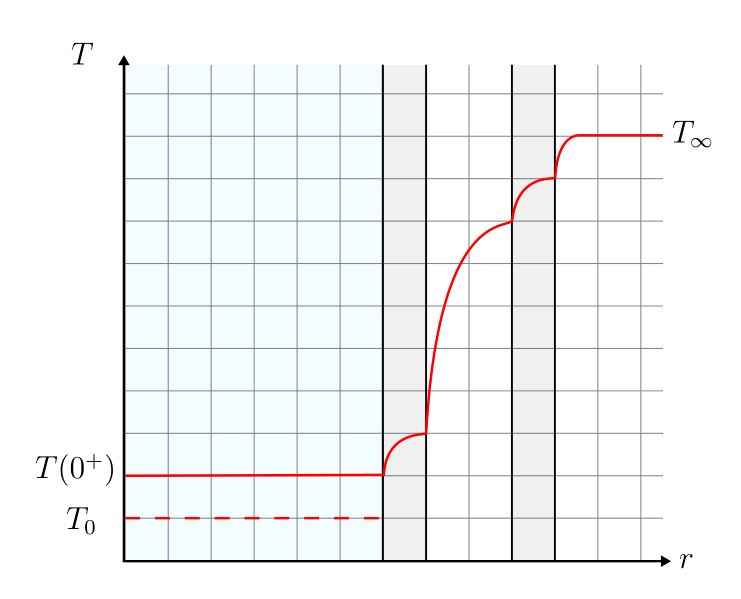
\includegraphics[width= 10cm]{tikz/15_3_2018_4a}
\end{figure}
\newline \\
b)\\ \\
Die Form des gesuchten Wärmedurchgangskoeffizienten kann der Formel \textit{Stationäre Wärmeleitung bei mehrschichtigem zylinderförmigem Wandaufbau} entnehmen und lautet somit
\[
	k(r) = \frac{1}{r}\frac{1}{\frac{1}{\lambda_w}\ln\left(\frac{r_i + w}{r_i}\right) + \frac{1}{\lambda_i}\ln\left(\frac{r_a - w}{r_i + w}\right) + \frac{1}{\lambda_w}\ln\left(\frac{r_a}{r_a - w}\right) + \frac{1}{r_a\alpha_\infty}}
\]
c)\\ \\
Die gesuchte Differentialgleichung lautet für $T(t)$
\[
	\frac{\text{d}}{\text{d}t}T(t) = -\frac{2k(r_i)}{\rho c_p r_i}(T(t) - T_\infty)
\]
d) \\ \\
Durch Lösen der obigen Differentialgleichung und einsetzen der gegebenen Bedingung erhält man die Zeit
\[
	t* = -\frac{\rho c_p r_i}{2k(r_i)}\ln\left(\frac{T* - T_\infty}{T_0 - T_\infty}\right)
\]
bei der die Flüssigkeit die gewünschte Temperatur erreicht hat.\\ \\